\documentclass[notitlepage]{article}
\usepackage[margin=0.75in]{geometry}
\usepackage{graphicx}
\author{Chris Manchester, Orren Saltzman}
\title{CIS 573 Project: Runtime Metamorphic Testing with Calico}
\parindent 0pt
\parskip 10pt

\begin{document}
\maketitle

\section{Introduction}

Calico is a C source code rewriter to be used to perform runtime metamorphic property testing on C programs. Calico takes as input a C source file, in which one or more functions has been annotated by the user according to a specified grammar (described below). This grammar conveys the metamorphic properties the function (or functions) is intended to have. Calico's output is a C program that behaves exactly as the original, except that each time an annotated function is called, it is called again with tranformed inputs, and the result is saved. The original output is also transformed, and it is asserted by the new program that the two results are equal. If they are, nothing has been proven about the correctness of the program, but if they are not, then the metamorphic property being asserted by the user has been violated, and the function under test has been to shown to be incorrect.

\begin{figure}[ht!]
\centering
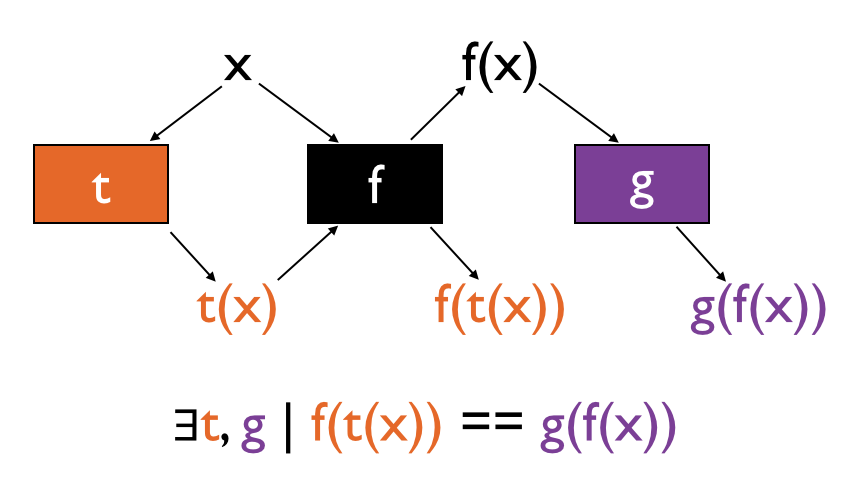
\includegraphics[width=175mm]{calico_pic1_alternate.png}
\caption{To specify a metamorphic property for the Function Under Test, f, the user must specify some functions t and g such that this equality holds.}
\end{figure}

\section{A Brief Description of Calico Instrumentation}

Many functions, particularly C functions, use side effects to accomplish their task. Furthermore, the data that might semantically be referred to as the ``result'' of a C function is not necessarily the same as the return value of that function. As such, it is necessary to assume that any piece of memory belonging to the process of the instrumented program might be considered $f(x)$ for the purpose of these assertions. Thus, it is neccessary to sandbox the effects of the function under test each time it is called, by spawning a new process for every additional time the function is called, times the number of properties being asserted. For instance, if a function is called by the application 100 times over the course of program execution, and three properties about the function are being specified, then the instrumented program must make 400 calls to the function: The original 100, plus 100 for each specified input transformation. For each of the 300 transformed calls, a process must be spawned and the result recovered by the main process through the use of shared memory. In this way, all side effects are sandboxed, and the entire application environment is held constant save the input to the function.

The form of the instrumented application is as follows:

\begin{figure}[ht!]
\centering
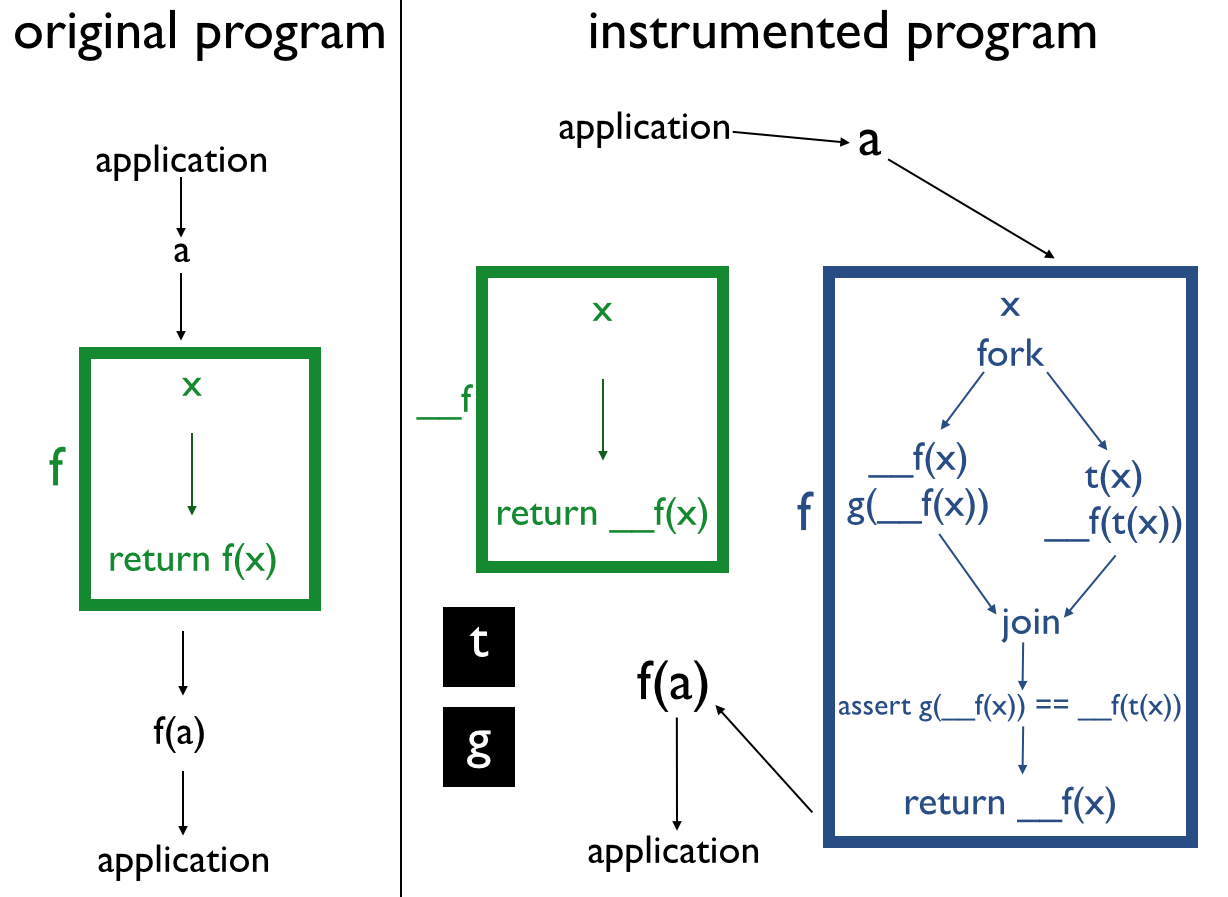
\includegraphics[width=175mm]{calico_pic2.png}
\caption{Calls to the function f are intercepted by a new function of the same name. The original is renamed with two leading underscores.}
\end{figure}

\section{The Annotation Language}

Annotations are placed in the comment text of a C function (above a function, between a /* and a */). Their form is as follows ({\bf ?} means 0 or 1 times, {\bf +} means 1 or more times, {\bf *} means 0 or more times{\bf}):

\ttfamily

<annotated-comment> ::= <unannotated-comment-text>{\bf ?} \\
\phantom{1}\hspace{120pt}<function-info-annotation> \\
\phantom{1}\hspace{120pt}<param-info-annotation>{\bf *} \\
\phantom{1}\hspace{120pt}<assertion-pair>{\bf +} \\

<function-info-annotation> ::= @fun-info { <function-name>, <function-kind>, <return-type> } ;

<function-kind> ::= ArithmeticReturn | PointerReturn | VoidReturn

<param-info-annotation> ::= @param-info { <C-identifier>, <param-type> } ;

<annotation-pair> ::= @input-prop <t-function>{\bf *} ; \\
\phantom{1}\hspace{110pt}@output-prop <g-function> ;

\rmfamily

\section{A short example: summing an array}

the following short file, called sum\_example.c, contains a function, sum, and a stub main function which simply calls sum on a toy array and prints the result:

\begin{verbatim}
#include <stdio.h>

extern void exit(int);

/**
 * May sum the elements of an array
 *
 * @fun-info { sum, "int" } ;
 * @param-info { arr, "int*" } ;
 * @param-info { length, "int" } ;
 * @input-prop { multiply_int_array(arr, 2, length), id } ;
 * @output-prop { double_int(result) } ;
 * @input-prop { duplicate(arr, length), double_int(length) } ;
 * @output-prop { double_int(result) } ;
 */
int sum ( int arr [], int length ) {
  int i = 0, r = 0;
  for (; i < length;) r += arr[i++];
  return r;
}

int main () {
  int arr [] = {1, 2, 3};
  int x = sum(arr, 3);
  printf("*** The sum is : %d\n", x);
  exit(0);
}
\end{verbatim}

the sum function has been annotated to assert two of its metamorphic properties. The first is that if you double each element of the input array, that the result will double. The second is that if you duplicate the array and use as input a new one which contains two copies of the original back to back, that the result will be doubled.

This source file is then instrumented by calcio, resulting in the following file, called calico\_gen\_sum\_example.c:

\begin{verbatim}
#include "calico_prop_library.h"
#include <stdio.h>

extern void exit(int);


/**
 * May sum the elements of an array
 *
 * @fun-info { sum, "int" } ;
 * @param-info { arr, "int*" } ;
 * @param-info { length, "int" } ;
 * @input-prop { multiply_int_array(arr, 2, length), id } ;
 * @output-prop { double_int(result) } ;
 * @input-prop { duplicate(arr, length), double_int(length) } ;
 * @output-prop { double_int(result) } ;
 */

int __sum( int arr [], int length ) {
  int i = 0, r = 0;
  for (; i < length;) r += arr[i++];
  return r;
}

int sum( int arr [], int length )  {
    int numProps = 2;
    size_t result_sizes[numProps];
    int* shmids = malloc(numProps * sizeof(int));
    int procNum = -1;
    int i;
    int *orig_result = malloc(sizeof(int));
    result_sizes[0] = sizeof(int);
    int* t_result0 = NULL;
    int* g_result0 = malloc(result_sizes[0]);

    result_sizes[1] = sizeof(int);
    int* t_result1 = NULL;
    int* g_result1 = malloc(result_sizes[1]);

    for (i = 0; i < numProps; i += 1) {
        if (procNum == -1) {
            if ((shmids[i] = shmget(key++, result_sizes[i], IPC_CREAT | 0666)) < 0) {
                perror("shmget");
                exit(1);
            }
            if (0 == fork()) {
                procNum = i;
                break;
            }
        }
    }

    if (procNum == -1) {
        *orig_result = __sum(arr, length);
        for (i = 0; i < numProps; i += 1) {
            wait(NULL);
        }
    }

    if (procNum == 0) {
        t_result0 = shmat(shmids[0], NULL, 0);
// < input_transformation
        multiply_int_array(arr, 2, length);
// input_transformation >;
        // < input_transformation
        ;
// input_transformation >// < call_inner_function
        *t_result0 = __sum(arr, length);
// call_inner_function >
        shmdt(t_result0);
        exit(0);
    }

    if (procNum == 1) {
        t_result1 = shmat(shmids[1], NULL, 0);
// < input_transformation
        arr = duplicate(arr, length);
// input_transformation >;
// < input_transformation
        length = double_int(length);
// input_transformation >// < call_inner_function
        *t_result1 = __sum(arr, length);
// call_inner_function >
        shmdt(t_result1);
        exit(0);
    }

    t_result0 = shmat(shmids[0], NULL, 0);
// < output_transformation
    *g_result0 = double_int(*orig_result);
// output_transformation >
    if (memcmp(g_result0, t_result0, sizeof(int))) {
        printf("a property has been violated:\ninput_prop: multiply_int_array, id\noutput_prop: double_int(result)\n");

    }

    t_result1 = shmat(shmids[1], NULL, 0);
// < output_transformation
    *g_result1 = double_int(*orig_result);
// output_transformation >
    if (memcmp(g_result1, t_result1, sizeof(int))) {
        printf("a property has been violated:\ninput_prop: duplicate, double_int\noutput_prop: double_int(result)\n");

    }

    free(shmids);
    return *orig_result;
}


int main () {
  int arr [] = {1, 2, 3};
  int x = sum(arr, 3);
  printf("*** The sum is : %d\n", x);
  exit(0);
}
\end{verbatim}

\section{Known Limitations/Future Work}

\subsection{probabalistic testing}

Instrumenting an application causes its runtime to increase, mostly due to the overhead of spawning new processes (The specific runtime costs associated with instrumentation are described in the next section). One feature that would allow the user to mitigate this problem would be to optionally accept a probability parameter through the annotation language. This probability, set to 1 by default, would determine the likelihood of a test being run each time a function under test is called by the application. In this way, the probability parameter can be fine-tuned such that performance comes back within whatever range is considered acceptable to the user. Because of the element of randomness in such a feature, a situation where certain kinds of inputs from the application are under-represented during testing would be unlikely, even though fewer total tests are being run.

\subsection{more sophisticated parsing methods}

The current implementation of calico does not go so far as to parse the entire C language. Instead, it parses the annotation language, and infers what it needs in terms of C source code from the location and content of the annotations. Future work on this project may include an attempt at a deeper parsing of the C grammar. This could potentially result in a somewhat simplified annotation language in which less information is required from the user.

\subsection{optimizations in memory management}

There is a certain subset of C functions which calico may not instrument in the optimal way from a memory management standpoint. Most notably, functions which perform side effects on large regions of memory, when instrumented, will create redundant copies of those regions using calls to memcpy. Changes could be made to calico's source translator that cause it to identify situations where those memcpy calls are not strictly necessary and direct subsequent reads of the data to the original result location, rather than a copied version.

Benefits of this feature in terms of space complexity would be linear with respect to the size of the inputs and outputs of the function under test. Benefits in terms of runtime complexity would be the same; however, the overhead of process spawning and deallocation is expected to be orders of magnitude more expensive than these calls to memcpy for the majority of applications, and so significant runtime gains should not be expected unless the input or output sizes are extremely large.

\section{Performance Measurement}

An experiment was run using a Machine Learning application called Martirank. Martirank contains an implementation of merge sort which takes as input the location of an array, and type and size information about the elements of that array. It then sorts the array in place.

This function was annotated to assert the following metamorphic property: If the elements of the input array are permuted, the resulting array should be the same. Note that because the array is sorted in-place, the ``result'' as we are choosing to think about it now is not the same as the return value of the function. This issue is dealt with using the optional \ttfamily @state-recover \rmfamily annotion described earlier.

Then, Martirank was run and timed with an example dataset. Then, an instrumented version was created and timed using the same dataset. The results are as follows:

\begin{tabular}{l | l | l}
& original & instrumented \\ \hline
calls to mergesort & $11047$ & $22094$ \\
total runtime (sec) & $.559$ & $24.403$ \\
new processes spawned & 0 & $11047$
\end{tabular}

Our resultant rough estimation of added runtime per assertion is $\frac{24.403}{11047} = {\mathbf .0022}$ seconds.

Note that the original runtime was not subracted from the total, since the experiment was run on a multi-core machine that parallelized the new calls with the old. Thus, the new calls are assumed to represent the main runtime bottleneck of the program.

\section{Calico's Implementation}

Calico is implemented in OCaml, a functional language well-suited to the task of source code rewriting. It consists of two main modules, calico/parser, which handles the C source inputs and parser them into the necessary data structure, and calcio/writer, the source code translator which takes that data structure and writes a new C source file.

\subsection{Description of the Parser}

\subsection{Description of the Source Translator}

\end{document}
